\sectionlink*{III. デコヒーレンス汎関数の端点項の評価}\label{sec:end_terms}

\begin{figure}[h!]
\centering
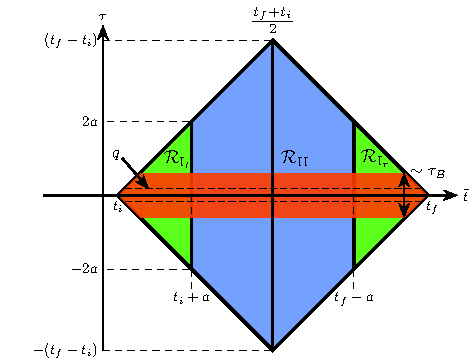
\includegraphics[width=.57\textwidth]{source/fig2.pdf}
\caption{本文の図\ref{fig1}に示した積分領域の、より詳細な模式図。部分領域 $\mathcal{R}_{\rm I}$ と $\mathcal{R}_{\rm II}$ を、それぞれ緑と青で示す。赤の領域は、FV 核 $k_r(\tau)$ が零でない台をもつ $(\tb,\tau)$ 平面の部分を表す。部分領域 $\mathcal{R}_{\rm II}$ では、$\tau$ の積分領域を無限大まで拡張し、本文と同様に扱うことができる。第 III 節では、$a$ によってパラメータ化された隅の領域 $\mathcal{R}_{{\rm I}_l}$ と $\mathcal{R}_{{\rm I}_r}$ の扱いを考える。試験関数 $x_{\tb}$ の、$a$ より短い時間尺度における変化は無視できるものと仮定する。}
\label{fig2}
\end{figure}

ここでは、本文の式\eqref{eq:decoh_action}で与えられるデコヒーレンス作用への端点項の寄与を、適切に扱うことを目指す。積分変数 $\tb$ と $\tau$ を用いると、この汎関数は
\be\label{eq:dec_func_end_terms}
	S_r[\Delta X] = \frac{1}{2}\iint_{\mathcal{R}_{\rm{I}} + \mathcal{R}_{\rm{II}}}d\tb\,d\tau\,k_r(\tau)\Delta X(\tb+\tau/2)\Delta X(\tb-\tau/2),
\ee
と書ける。ここで $\mathcal{R}_{\rm{I}/\rm{II}}$ は、図\ref{fig2}に緑と青で示した領域を定義する：
\begin{align*}
	&\mathcal{R}_{\rm I} = \mathcal{R}_{{\rm I}_l} \cup \mathcal{R}_{{\rm I}_r}\\
	&\qquad \mathcal{R}_{{\rm I}_l} = \{(\tb,\tau) :  t_i\leq \tb\leq t_i+a, \, -2(\tb-t_i)\leq\tau\leq 2(\tb-t_i)\} \\
	&\qquad \mathcal{R}_{{\rm I}_r} = \{(\tb,\tau) :  t_f-a\leq \tb\leq t_f, \, -2(t_f-\tb)\leq\tau\leq 2(t_f-\tb)\} \\
	&\text{および} \\
	&\mathcal{R}_{\rm II} = \mathcal{R}_{{\rm II}_l} \cup \mathcal{R}_{{\rm II}_r}\\
	&\qquad \mathcal{R}_{\rm {II}_l} = \{(\tb,\tau) : t_i+a\leq \tb\leq \frac{1}{2}(t_f+t_i), \, -2(\tb-t_i)\leq\tau\leq 2(\tb-t_i)\}  \\
	&\qquad \mathcal{R}_{\rm {II}_r} = \{(\tb,\tau) : \frac{1}{2}(t_f+t_i)\leq \tb\leq t_f-a, \, -2(t_f-\tb)\leq\tau\leq 2(t_f-\tb)\}.
\end{align*}
パラメータ $a$ は、端点 $t_i$ および $t_f$ に対する領域 $\mathcal{R}_{\rm II}$ の境界を定める。$a\gtrsim\tau_B$ を満たすように $a$ を固定すれば、赤の領域と比べて有意な寄与を拾うことがないため、$\mathcal{R}_{\rm II}$ における $\tau$ の積分範囲を実数直線全体まで拡張できる。また、この領域のパラメータ $q$ も、第 II 節と同様に任意に小さくできる。したがって、対応するデコヒーレンス汎関数は、$\tb$ の積分範囲を変更した、本文の式\eqref{eq:action}と同じ形をとる：
\begin{align}
	S^{\rm II}_r[\Delta X] &= \frac{1}{2}\int^{t_f-a}_{t_i+a}d\tb\int^{\infty}_{-\infty}d\tau\,k_r(\tau)\Delta X(\tb+\tau/2)\Delta X(\tb-\tau/2) \nonumber\\
		    &= \frac{2\eta}{\pi}\int^{t_f-a}_{t_i+a}d\tb\left[\frac{\pi}{\tau_B} \Delta X^2(\tb) + \int^{\infty}_0d\tau\,k^{(m)}_r(\tau)(\Delta X^2(\tb) - \Delta X(\tb+\tau/2)\Delta X(\tb-\tau/2))\right],
\end{align}
これは高温極限で
\be\label{eq:dec_func_II_htl}
	S^{\rm II}_r[\Delta X] \approx \frac{2\eta}{\tau_B}\int^{t_f-a}_{t_i+a}d\tb\,\Delta X(\tb)^2 + \frac{\eta\tau_B}{12}\int^{t_f-a}_{t_i+a}d\tb\,\Big(\Delta X'(\tb)^2 - \Delta X(\tb)\Delta X''(\tb)\Big).
\ee
となる。次に部分領域 $\mathcal{R}_{\rm I}$ を考えると、それぞれの隅の区分 $\mathcal{R}_{{\rm I}_l}$ および $\mathcal{R}_{{\rm I}_r}$ 内のデコヒーレンス作用は
\begin{subequations}
\begin{align}
    S^{{\rm I}_l}_r[\Delta X] &= \frac{1}{2}\int^{t_i+a}_{t_i}d\tb\int^{2(\tb-t_i)}_{-2(\tb-t_i)}d\tau\,k_r(\tau)\Delta X(\tb+\tau/2)\Delta X(\tb-\tau/2), \label{eq:decoh_action_l} \\
    S^{{\rm I}_r}_r[\Delta X] &= \frac{1}{2}\int^{t_f}_{t_f-a}d\tb\int^{2(t_f-\tb)}_{-2(t_f-\tb)}d\tau\,k_r(\tau)\Delta X(\tb+\tau/2)\Delta X(\tb-\tau/2). \label{eq:decoh_action_r}
\end{align}
\end{subequations}
で与えられる。各 $\tb$ 積分に対する、端点 $t_i$ および $t_f$ 近傍からの寄与を分離して、
\begin{subequations}
\begin{align}
    S^{{\rm I}_l}_r[x] &= \bar{S}^{{\rm I}_l}_r[x] + R^{{\rm I}_l}_r[x], \\
    S^{{\rm I}_r}_r[x] &= \bar{S}^{{\rm I}_r}_r[x] + R^{{\rm I}_r}_r[x],
\end{align}
\end{subequations}
とする。ここで、
\begin{subequations}
\begin{align}
    R^{{\rm I}_l}_r[x] &:= \frac{\eta}{\pi\tau_B}\int^{t^+_i}_{t_i}d\tb\int^{\frac{2(\tb - t_i)}{\tau_B}}_{\frac{-2(\tb - t_i)}{\tau_B}}ds\,F_{\Lambda}(s)x_{\tb}(s), \label{eq:R_left}\\
    R^{{\rm I}_r}_r[x] &:= \frac{\eta}{\pi\tau_B}\int^{t_f}_{t^-_f}d\tb\int^{\frac{2(t_f - \tb)}{\tau_B}}_{\frac{-2(t_f - \tb)}{\tau_B}}ds\,F_{\Lambda}(s)x_{\tb}(s),\label{eq:R_right}
\end{align}
\end{subequations}
は剰余項を定義する。左の隅の領域に対する剰余は、
\begin{align}
    \left|\int^{t^+_i}_{t_i} d\tb\int^{\frac{2(\tb - t_i)}{\tau_B}}_{-\frac{2(\tb - t_i)}{\tau_B}} ds\,F_{\Lambda}(s)x_{\tb}(s)\right| &\leq \int^{t^+_i}_{t_i} d\tb\int^{\frac{2(\tb - t_i)}{\tau_B}}_{-\frac{2(\tb - t_i)}{\tau_B}} ds\,|F_{\Lambda}(s)x_{\tb}(s)| \nonumber\\
    &\leq M_{\Lambda}\int^{t^+_i}_{t_i} d\tb\int^{\frac{2(\tb - t_i)}{\tau_B}}_{-\frac{2(\tb - t_i)}{\tau_B}}ds \nonumber\\
    &= 2M_{\Lambda}\frac{\delta t^2}{\tau_B},
\end{align}
から評価できる。ここで $M_{\Lambda} := \sup_{\tb,s\in\mathcal{R}_{{\rm I}_l}}|F_{\Lambda}(s)x_{\tb}(s)|$、$\delta t := t^+_i-t_i$ である。これより、
\be
    |R^{{\rm I}_l}_r| \leq \frac{2\eta M_{\Lambda}}{\pi}\frac{\delta t^2}{\tau^2_B},
\ee
が得られるので、$\delta t \ll \sqrt{\pi\tau^2_B/2\eta M_{\Lambda}}$ である限り、$R^{{\rm I}_l}_r[x]$ を小さくできる。同様の解析は $R^{{\rm I}_r}_r[x]$ にも適用できる。

次に作用汎関数 $\bar{S}^{{\rm I}_{l/r}}_r[\Delta X]$ に着目すると、式\eqref{eq:decoh_action_l}および\eqref{eq:decoh_action_r}の内側の積分は、第 II 節で述べたものと同じ手順に従って評価できる。その結果、
\begin{subequations}
\begin{align}
	\bar{S}^{{\rm I}_l}_r[\Delta X] &= \frac{2\eta}{\tau_B}\int^{t_i+a}_{t^+_i}d\tb\,\coth\left(\frac{2\pi(\tb-t_i)}{\tau_B}\right)\Delta X(\tb)^2 \nonumber\\
		      &\qquad + \frac{2\eta}{\pi}\int^{t_i+a}_{t^+_i}d\tb \int^{2(\tb-t_i)}_qd\tau\,k^{(m)}_r(\tau)\big(\Delta X^2(\tb) - \Delta X(\tb + \tau/2)\Delta X(\tb - \tau/2)\big), \label{eq:S_I_left}\\
	\bar{S}^{{\rm I}_r}_r[\Delta X] &= \frac{2\eta}{\tau_B}\int^{t^-_f}_{t_f-a}d\tb\,\coth\left(\frac{2\pi(t_f-\tb)}{\tau_B}\right)\Delta X(\tb)^2 \nonumber\\
		      &\qquad + \frac{2\eta}{\pi}\int^{t^-_f}_{t_f-a}d\tb \int^{2(t_f-\tb)}_qd\tau\,k^{(m)}_r(\tau)\big(\Delta X^2(\tb) - \Delta X(\tb + \tau/2)\Delta X(\tb - \tau/2)\big). \label{eq:S_I_right}
\end{align}
\end{subequations}
を得る。式\eqref{eq:T_lim}と異なり、$\tau$ 積分の極限 $q\rightarrow0$ を形式的にとることはできない点に注意されたい。$\lim_{\Lambda\rightarrow\infty}M_{\Lambda}=\infty$ であり、そのため剰余項 $R^{{\rm I}_{l/r}}_r[x]$ を適切に有界に保てなくなるからである。ただし、$q$ が十分小さい（あるいは $\Lambda$ が十分大きい）と仮定して、これらの積分の下限を近似的に零にすることはできる。

ここで高温極限を考える。式(\ref{eq:S_I_left})および(\ref{eq:S_I_right})の内側の項を $\tau$ の最低次まで展開すると、
\begin{subequations}
\begin{align}
	\bar{S}^{{\rm I}_l}_r[\Delta X] &\approx \Big(\dots\Big) + \frac{2\tau_B\eta}{\pi^2}\int^{t_i+a}_{t^+_i}d\tb\, B\left(\frac{2\pi(\tb-t_i)}{\tau_B}\right)\big(\Delta X'(\tb)^2 - \Delta X(\tb)\Delta X''(\tb)\big), \label{eq:S_I_l_htl} \\
	\bar{S}^{{\rm I}_r}_r[\Delta X] &\approx\Big(\dots\Big) + \frac{2\tau_B\eta}{\pi^2}\int^{t^-_f}_{t_f-a}d\tb\,B\left(\frac{2\pi(t_f-\tb)}{\tau_B}\right)\big(\Delta X'(\tb)^2 - \Delta X(\tb)\Delta X''(\tb)\big), \label{eq:S_I_r_htl}
\end{align}
\end{subequations}
となる。ここで $B(t)$ は、核 $k^{(m)}_r(\tau)$ の原始関数として
\be\label{eq:B}
	B\Big(\frac{\pi t}{\tau_B}\Big) := \frac{\pi}{\tau_B}\int^t_0d\tau\,k^{(m)}_r(\tau) = \int^{\frac{\pi t}{\tau_B}}_0dx\,x^2\csh^2x .
\ee
によって定義される。この積分の解析的な結果は、
\be\label{eq:B_scaled}
        B(t) = t\big[t - t\coth{t} + 2\ln(1-e^{-2t})\big] - {\rm Li}_2(e^{-2t}) + \frac{\pi^2}{6},
\ee
と求められる。ここで ${\rm Li}_s(t) = \sum^{\infty}_{k=1}\frac{t^k}{k^s}$ は多重対数関数である。

図\ref{fig3}には、$\tau_B$ のいくつかの値に対して積分 $B(\pi t/\tau_B)$ を示している。逆時間 $\tau^{-1}_B$ は、積分が漸近値に達する速さを決定する。したがって、$\tau_B$ が十分小さいとき、式(\ref{eq:S_I_left})の内側の積分は、境界 $t_i$ に近いものを除くほぼすべての $\tb$ の値について一定となる。$\tb$ が上限 $t_f$ に近づく場合の式(\ref{eq:S_I_right})の内側の積分についても、同じことが当てはまる。

\begin{figure}[t!]
\centering
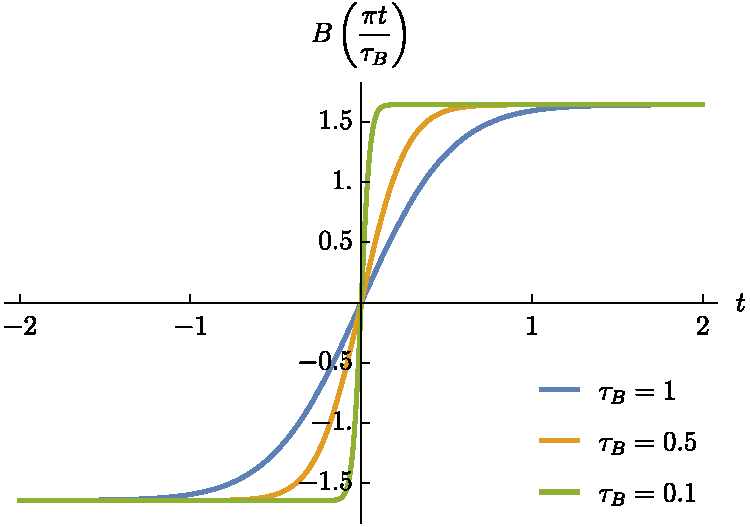
\includegraphics[width=.5\textwidth]{source/fig3.pdf}
\caption{\label{fig3} $t$ によって定まる上限を変化させたときの積分(\ref{eq:B})のプロット。$t\rightarrow\infty$ で値 $\frac{\pi^2}{6}$ に漸近する。式(\ref{eq:B_scaled})を参照。}
\end{figure}

この振る舞いは次のように定式化できる。$\mu(\tb)$ により測度を区分的に
\begin{align}
	d\mu(\tb) =
	\begin{cases}
		d\tb \qquad\qquad  & \tb\in(t_i+m, t_f-m\tau_B), \\
		\frac{6}{\pi^2}B\left(\frac{\tb-t_i}{\tau_B}\right)d\tb \qquad\qquad & \tb\in[t_i, t_i+m\tau_B], \\
		\frac{6}{\pi^2}B\left(\frac{t_f-\tb}{\tau_B}\right)d\tb \qquad\qquad  & \tb\in[t_f-m\tau_B, t_f],
	\end{cases}
\end{align}
と定義する。ここで $m\in\mathbb{R}^+$ は $B(m\tau_B/\pi)\sim \frac{\pi^2}{6}$ を満たすように選ぶ。このとき $\tau_B\rightarrow0$ とすると、$B(\pi t/\tau_B)$ が $\frac{\pi^2}{6}$ からずれる領域は、区間 $[t_i,t_f]$ の端点に限定される。これらの点の測度は零であるから、
\be\label{eq:int_measure}
	\lim_{\tau_B\rightarrow0}d\mu(\tb) =
	\begin{cases}
		d\tb \qquad &\tb\in(t_i,t_f), \\
		0, \qquad &\tb\in\{t_i,t_f\},
	\end{cases}
\ee
が成り立つ。$\mu(\tb)$ の極限での振る舞いを図\ref{fig4}に示す。

\begin{figure}[t!]
\centering
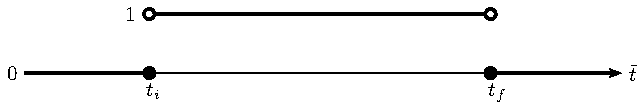
\includegraphics[width=.6\textwidth]{source/fig4.pdf}
\caption{\label{fig4} 高温極限において区間 $[t_i, t_f]$ に作用する積分測度 $d\mu(\tb)$。}
\end{figure}

式(\ref{eq:S_I_l_htl})および(\ref{eq:S_I_r_htl})はすでに $\tau_B$ が小さい極限で展開されているため、
\begin{align}\label{eq:dec_func_result}
	S_r[\Delta X] &= S^{\rm I}_r[\Delta X] + S^{\rm II}_r[\Delta X] \nonumber\\
	      &\approx \frac{2\eta}{\tau_B}\bigg[\int^{t_f-a}_{t_i+a}d\tb\,\Delta X(\tb)^2  \nonumber \\
	      &\qquad + \int^{t_i+a}_{t^+_i}d\tb\,\coth\left(\frac{2\pi(\tb-t_i)}{\tau_B}\right)\Delta X(\tb)^2 + \int^{t^-_f}_{t_f-a}d\tb\,\coth\left(\frac{2\pi(t_f-\tb)}{\tau_B}\right)\Delta X(\tb)^2\bigg] \nonumber\\
	      &\qquad + \frac{\eta\tau_B}{12}\int^{t_f}_{t_i}d\mu(\tb)\big(\Delta X'(\tb)^2 - \Delta X(\tb)X''(\tb)\big) + R^{{\rm I}_l}_r[\Delta X] + R^{{\rm I}_r}_r[\Delta X].
\end{align}
と書ける。さらに、同じ極限で
\begin{align*}
    &\lim_{\tau_B\rightarrow0}\coth\left(\frac{2\pi(\tb-t_i)}{\tau_B}\right) = 1 \qquad \tb\in(t_i,t_i+a), \\
    &\lim_{\tau_B\rightarrow0}\coth\left(\frac{2\pi(t_f-\tb)}{\tau_B}\right) = 1 \qquad \tb\in(t_f-a,t_f),
\end{align*}
に注意すると、式\eqref{eq:dec_func_result}の第1行と第2行も測度 $d\mu(\tb)$ を用いて次のように書ける：
\be
    S_r[\Delta X] \approx \int^{t_f}_{t_i}d\mu(\tb)\bigg[\frac{2\eta}{\tau_B}\Delta X^2(\tb) + \frac{\eta\tau_B}{12}\big(\Delta X'(\tb)^2 - \Delta X(\tb)\Delta X''(\tb)\big)\bigg] + R^{{\rm I}_l}_r[\Delta X] + R^{{\rm I}_r}_r[\Delta X].
\ee
したがって、デコヒーレンス汎関数 $S_r[\Delta X]$ の端点項を明示的に扱うことにより、剰余項を無視できるほど小さくできるならば、本文の式\eqref{eq:action}--\eqref{eq:decoh_action_1}と同様の結果が得られる。
